
\section{Data analytics with Waziup platform}

\begin{figure}[htb]  
\centering  
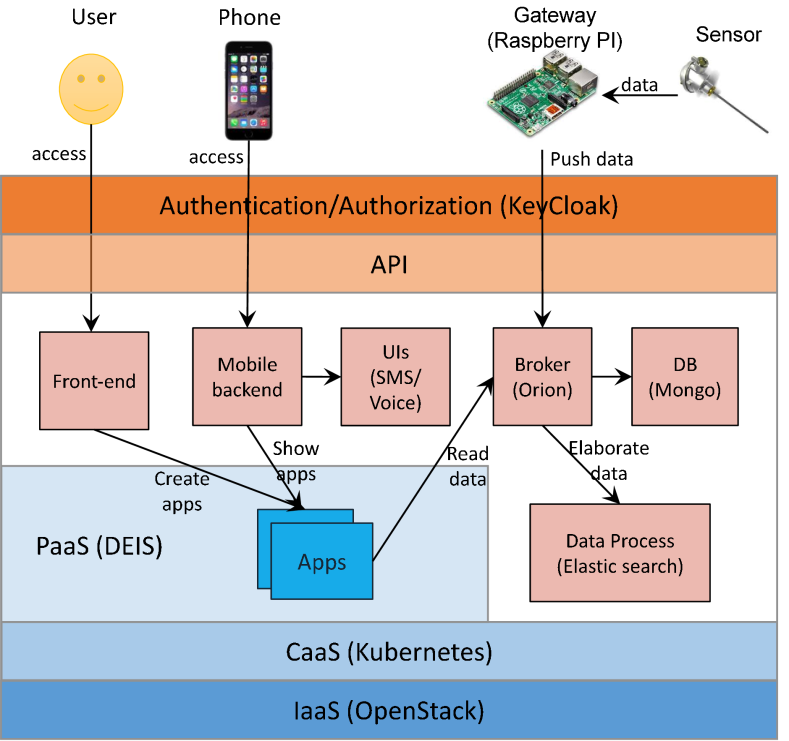
\includegraphics[width=.6\linewidth]{figures/implem}   
\caption{Cloud platform implementation}
\label{fig-implem}  
\end{figure} 

The Figure~\ref{fig-implem} presents the implementation of the Waziup platform stack.
The role of each component is presented, together with the technology selected in parenthesis.
The Waziup platform uses three distinct Cloud layers (in blue in the picture):
\begin{enumerate}
  \item “Infrastructure as a Service” (IaaS),    
  \item “Container as a Service” (CaaS),    
  \item and finally “Platform as a Service” (PaaS).     
\end{enumerate}

The first layer is provided by OpenStack.
Its main role is to provide Virtual Machines (VMs), in which we run the full platform.
This layer is fundamental because most of Cloud vendors (Amazon, Rackspace…) use VMs as basic selling units.
The second layer is provided by Kubernetes.
The role of this layer is to provide containers, such as Docker containers.
These containers provide light-weight and ultra-fast virtualization for applications and micro-services.
The containers themselves are running inside the VMs.
The third and final Cloud layer is provided by Deis.
It provides services to developers, such as compiling and deploying an application.
All the applications pushed by the users will be compiled with Deis and hosted in containers on Kubernetes.

To access the platform, the users and external components need to go through the API server.
The API server exposes a common API for all the services of the Waziup platform.
Each of the endpoints of the API server is secured with Keycloak.

Keycloak provides both Authentication and Authorization management.
For instance, when accessing the dashboard, the user need to provide a username and password.
This is provided by Keycloak authentication layer.
Furthermore, through the dashboard and APIs the user can access only sensors that are authorized for him.
This is enforced by Keycloak authorization layer.

Mobile phones are used to interfaces with the SMS and voice commands component.
This component allows Waziup applications to send SMS and voice notifications to the users.
The Gateway pushes sensors' data to the data broker, which is FIWARE Orion.
The data is distributed to the applications requesting it.
Orion also interfaces with the database and the data processing (Elastic Search), for historical data analysis.
In this section we will present WAZIUP platform components and the technology and tools selected for each component.


